\documentclass[a4paper]{article}
%~~~~~~~~~~~~~~~~~~~~~~~~~~~~~Packages~~~~~~~~~~~~~~~~~~~~~~~~~~~~%
\usepackage[english]{babel}
\usepackage[utf8x]{inputenc}
\usepackage{booktabs}
\usepackage{tabu}
\usepackage{cancel}
%% Sets page size and margins
\usepackage[a4paper,top=2cm,bottom=2cm,left=2cm,right=2cm,marginparwidth=1.75cm]{geometry}
\usepackage{amsmath}
\usepackage{enumitem}
\usepackage{listings}
\usepackage{subfigure}
\usepackage{relsize}
\usepackage{graphicx}
%\usepackage{apacite}
\usepackage{pgfplots}
\usepackage{comment}
\usepackage[colorinlistoftodos]{todonotes}
\usepackage[colorlinks=true, allcolors=blue]{hyperref}

%~~~~~~~~~~~~~~~~~~~~~~~~~~~~~Commands~~~~~~~~~~~~~~~~~~~~~~~~~~~~%

\renewcommand{\abstractname}{Summary}

%~~~~~~~~~~~~~~~~~~~~~~~~~~~~~pgfPlots~~~~~~~~~~~~~~~~~~~~~~~~~~~~%

\pgfplotsset{compat=1.8}
\usepgfplotslibrary{statistics}
%%%%%%%%%%%%%%%%%%%%%%%%%%%%%%%%%%%%%%%%%%%%%%%%%%%%%%%%%%%%%%%%%%%%

\begin{document}

\begin{titlepage}
\begin{center}
\vspace{3cm}

\Large

\vspace{2cm}

  
\includegraphics[scale=0.3]{imgs/Cherubino.jpg}

\vspace{2.5cm}

{\Huge \sc Data mining project report}

\vspace{1cm}

Maddalena Amendola

\vspace{1cm}

Daniele Gadler

\vspace{1cm}

Riccardo Manetti

\vspace{1cm}

Gemma Martini

\vfill

\today

\end{center}
\end{titlepage}

%%%%%%%%%%%%~~~~~~~~~~~~~~~~~~~~~~~~~~~~~~~~~~~~~~~~~~~%%%%%%%%%%%%

\tableofcontents
\newpage

%%%%%%%%%%%%%%~~~~~~~~~~~~~~~~~~~~~~~~~~~~~~~~~~~~~~~~~~~%%%%%%%%%%
%\author{  Group 1\\ Amendola Maddalena, Daniele Gadler, Gemma Martini, Riccardo Manetti  \\Department of Computer Science, University of Pisa \\ \date{ 1nd Semester of Academic Year 2018--2019}

%\begin{abstract}
 %  This is the abstract text
%\end{abstract}


\section{Data Understanding}

This part contains a first analysis of the data contained in the credit card dataset.

\subsection{BoxPlots by Gemma}

\subsubsection{Age}
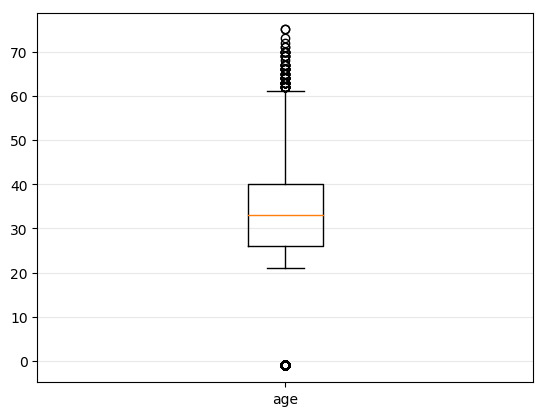
\includegraphics[width=0.9\textwidth]{../Code/boxPlotsGemma/boxplots/age.png}


\subsubsection{Limit}
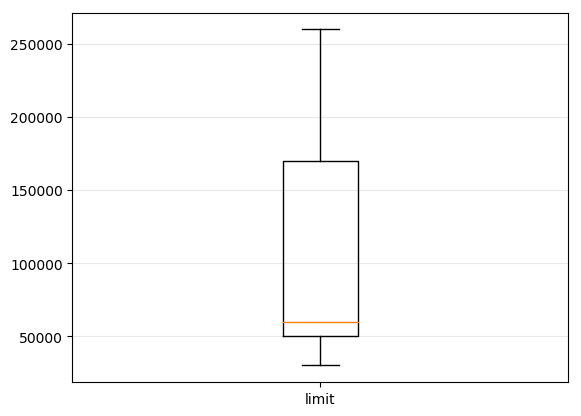
\includegraphics[width=0.9\textwidth]{../Code/boxPlotsGemma/boxplots/limit.png}


\subsubsection{ba}
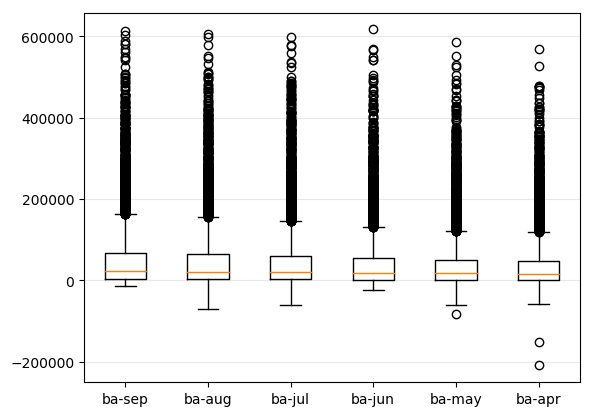
\includegraphics[width=0.9\textwidth]{../Code/boxPlotsGemma/boxplots/ba.png}


\subsubsection{pa}
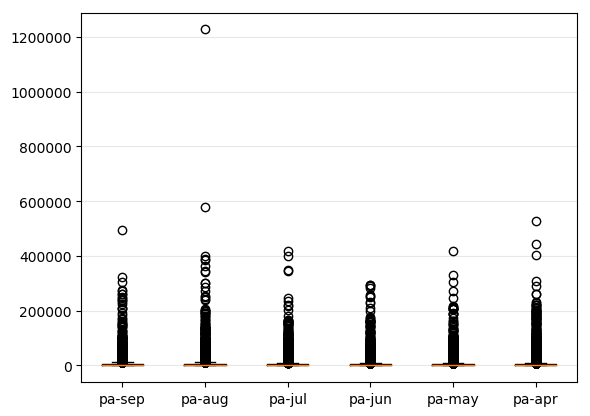
\includegraphics[width=0.9\textwidth]{../Code/boxPlotsGemma/boxplots/pa.png}


\subsubsection{ps}
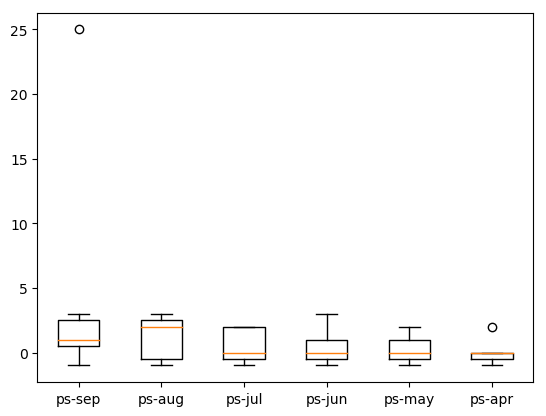
\includegraphics[width=0.9\textwidth]{../Code/boxPlotsGemma/boxplots/ps.png}


\bibliographystyle{plain}
\bibliography{bibtex}

\end{document}
              
